\documentclass[12pt, a4paper]{article}

% Avoid useless warnings about included images
% Reference: https://tex.stackexchange.com/a/78020
%\pdfsuppresswarningpagegroup=1

% Use \hypersetup here to get rid of the ugly boxes around links
\usepackage{hyperref}
\hypersetup{
  colorlinks=true,
  linkcolor=blue,
  urlcolor=blue
}

% Avoid warning about missing font for \textbackslash character.
\usepackage[T1]{fontenc}

% For nicer paragraph spacing
\usepackage{parskip}

\usepackage[disable]{todonotes}
%\usepackage{todonotes}

\usepackage{amsmath}%
\usepackage{amsfonts}%
\usepackage{amssymb}%
\usepackage{graphicx}
%\usepackage[miktex]{gnuplottex}
%\ShellEscapetrue
\usepackage{epstopdf}
\usepackage{longtable}
\usepackage{floatrow}
\usepackage{makecell}

% Use \setminted here to get horizontal line above and below listings
\usepackage[cache=false]{minted}
\setminted{
   frame=lines,
   framesep=2mm
}

\usepackage{textcomp}
\usepackage{color,soul}
\usepackage[font={small,it}]{caption}
\floatsetup[listing]{style=Plaintop}    
\floatsetup[longlisting]{style=Plaintop}    

% Turn off indentation but allow \indent command to still work.
\newlength\tindent
\setlength{\tindent}{\parindent}
\setlength{\parindent}{0pt}
\renewcommand{\indent}{\hspace*{\tindent}}

\addtolength{\textwidth}{0.8in}
\addtolength{\oddsidemargin}{-.4in}
\addtolength{\evensidemargin}{-.4in}
\addtolength{\textheight}{1.6in}
\addtolength{\topmargin}{-.8in}

\usepackage{longtable,supertabular}
\usepackage{listings}
\lstset{
  frame=top,frame=bottom,
  basicstyle=\ttfamily,
  language=XML,
  tabsize=2,
  belowskip=2\medskipamount
}

% All listings have a left aligned caption. This looks better as the listings themselves are left aligned.
\captionsetup[listing]{justification=justified,singlelinecheck=false}

\usepackage{tabu}
\tabulinesep=1.0mm
\restylefloat{table}

\usepackage{siunitx}

\newenvironment{longlisting}{\captionsetup{type=listing}}{}
%\usepackage[colorlinks=true]{hyperref}

% Inline code fragments can run over the page boundary without ragged right.
\AtBeginDocument{\raggedright}

\renewcommand\P{\ensuremath{\mathbb{P}}}
\newcommand\E{\ensuremath{\mathbb{E}}}
\newcommand\Q{\ensuremath{\mathbb{Q}}}
\newcommand\I{\mathds{1}}
\newcommand\F{\ensuremath{\mathcal F}}
\newcommand\V{\ensuremath{\mathbb{V}}}
\newcommand\YOY{{\rm YOY}}
\newcommand\Prob{\ensuremath{\mathbb{P}}}
\newcommand{\D}[1]{\mbox{d}#1}
\newcommand{\NPV}{\mathit{NPV}}
\newcommand{\CVA}{\mathit{CVA}}
\newcommand{\DVA}{\mathit{DVA}}
\newcommand{\FVA}{\mathit{FVA}}
\newcommand{\COLVA}{\mathit{COLVA}}
\newcommand{\FCA}{\mathit{FCA}}
\newcommand{\FBA}{\mathit{FBA}}
\newcommand{\KVA}{\mathit{KVA}}
\newcommand{\MVA}{\mathit{MVA}}
\newcommand{\PFE}{\mathit{PFE}}
\newcommand{\EE}{\mathit{EE}}
\newcommand{\EPE}{\mathit{EPE}}
\newcommand{\ENE}{\mathit{ENE}}
\newcommand{\EEPE}{\mathit{EEPE}}
\newcommand{\EEE}{\mathit{EEE}}
\newcommand{\EAD}{\mathit{EAD}}
\newcommand{\PE}{\mathit{PE}}
\newcommand{\NE}{\mathit{NE}}
\newcommand{\RC}{\mathit{RC}}
\newcommand{\RW}{\mathit{RW}}
\newcommand{\NS}{\mathit{NS}}
\newcommand{\PD}{\mathit{PD}}
\newcommand{\LGD}{\mathit{LGD}}
\newcommand{\DIM}{\mathit{DIM}}
\newcommand{\DF}{\mathit{DF}}
\newcommand{\MA}{\mathit{MA}}
\newcommand{\SCVA}{\mathit{SCVA}}
\newcommand{\bs}{\textbackslash}
\newcommand{\REDY}{\color{red}Y}

\begin{document}

\title{Open Source Risk Engine \\ Design}
\author{Acadia Inc.}
\maketitle

\newpage

%-------------------------------------------------------------------------------
\section*{Document History}

\begin{center}
\begin{supertabular}{|l|l|p{9cm}|}
\hline
Date & Author & Comment \\
\hline
14 November 2019 & Roland Lichters & initial release\\
\hline
4 December 2021 & Roland Kapl & enhancements and new developments of 1.6\\
\hline
\end{supertabular}
\end{center}

\newpage

\tableofcontents
\newpage

\section{Introduction}

Open Source Risk Engine (ORE, \url{https://opensourcerisk.org}) was first released by Quaternion (\url{https://www.quaternion.com}) as free/open-source software in 2016, with six subsequent releases to date, the latest version as of July 2021. 

The Open Source Risk project aims at establishing a transparent peer-reviewed framework for pricing and risk analysis that serves as

\begin{itemize}
\item a benchmarking, validation, training, teaching reference
\item an extensible foundation for tailored risk solutions.
\end{itemize}

ORE's analytics cover
\begin{itemize}
\item Financial instrument valuation for a range of derivatives products and bonds across six risk classes - interest rates, foreign exchange, inflation, equity, credit and commodity
\item market risk analysis, sensitivity analysis, stress testing, Value at Risk
\item credit exposure simulation
\item CSA pricing and XVA calculation
\end{itemize}

ORE is based on QuantLib (\url{https://quantlib.org}), the ``free/open-source library for quantitative finance'', which in turn depends on the Boost C++ libraries (\url{https://boost.org}). 
The QuantLib project had its initial release in December 2000, and it has grown over almost two decades to about 420 thousand lines of code, driven by a small number of ``authors'' and larger number of ``contributors'', including a number of Quaternion staff.

QuantLib provides the ``infrastructure'' of a fundamental class hierarchy covering dates and date arithmetic, calendars, schedules and schedule generation from rules, yield/inflation/default term structures and bootstrap methods,
Financial instruments, models and model calibration, pricing engines, various pricing method templates (analytical, Monte Carlo simulation, finite difference), and a range of underlying mathematical utilities including solvers, optimizers, interpolators etc.

ORE extends QuantLib, adding to QuantLib's class hierarchy what we have experienced as missing ingredients in our history as QuantLib users over the past 15 years.
Moreover, and in contrast to QuantLib, ORE provides a risk application that is designed to be accessible to end users, providing

\begin{itemize}
\item a simple command-line application with input/output files
\item transparent interfaces for trade data, market data, system configuration
\item a detailed user guide with a large range of examples of ORE usage, see \url{https://opensourcerisk.org/documentation}
\end{itemize}

The purpose of this document is describing the layout and technical design of ORE, as well as its connection with QuantLib.


\section{Overview}
Like QuantLib, ORE is written in C++, and it is organized in a hierarchy of C++ libraries an application needs to be linked with, as indicated in figure \ref{fig_Hierarchy}.

\begin{figure}[h]
\begin{center}
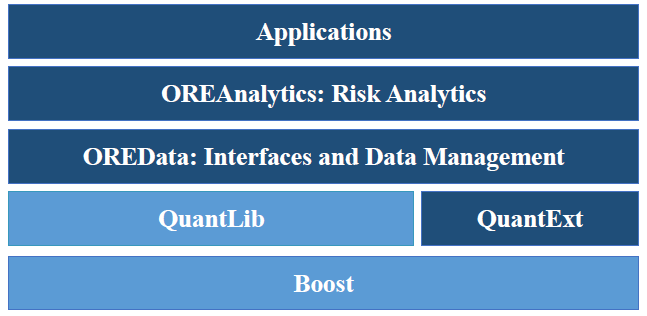
\includegraphics[scale=0.6]{Overview}
\end{center}
\caption{Hierarchy of ORE libraries. }
\label{fig_Hierarchy}
\end{figure}

The dark blue parts of indicate components of ORE, dependencies are indicated in light blue color.

\subsection*{QuantExt - Collection of QuantLib Extensions}

Extensions to QuantLib such as financial instruments, pricing models, pricing engines and term structures are collected in the QuantExt library. 
The internal organization of QuantExt (folder structure, class hierarchy) mimics the structure of QuantLib, so that a developer who is familiar with QuantLib will have little difficulty finding her/his way around QuantExt as well.

At an early stage of the Open Source Risk project we decided to keep these kind of extensions separate from QuantLib (rather than adding to a local copy of the QuantLib library or immediately contributing these changes to the QuantLib project).
This facilitates QuantLib release changes, swapping QuantLib in ORE for another/newer version of QuantLib.

Similarly, rather than patching a copy of QuantLib locally when identifying a bug or issue, we tend to copy the affected QuantLib class or part of the QuantLib class hierarchy to QuantExt and apply the correction in QuantExt. In doing so, we decouple
from the QuantLib release cycle and bug fixes and facilitate quick fixes of parts of QuantLib that ORE critically depends on.

Some of the extensions that go into QuantExt may be contributed back into QuantLib with a delay, and then removed from QuantExt again. Examples are cross currency instruments and related engines and bootstrap helpers. Other extensions that are more
relevant for the risk analytics in ORE may stay in QuantExt longer term, such as the cross asset model underlying the Monte Carlo scenario generation for exposure simulation and xVA in ORE.

QuantLib's focus is on the individual instrument and its valuation and analysis whereas ORE aims at portfolio analytics that may be more than simply additive in the instrument's contributions (such as xVA, Value at Risk, etc). QuantExt provides
models and methods to support these analytics so that we might see QuantExt existing in parallel to QuantLib in the longer term.

\subsection*{OREData - Data Management, Translation and Assembly}

OREData is a library beyond the scope of QuantLib and QuantExt. OREData serves at the high level two purposes summarized under the label of ``data management''
\begin{itemize}
\item to {\bf translate} between external (XML) representations of financial objects and internal (C++) representations of objects in memory that QuantLib and QuantExt can deal with
\item to {\bf assemble essential object hierarchies} underneath the abstract
\begin{itemize}
\item {\bf Portfolio} object containing pointers to all financial products ``loaded''
\item {\bf Market} objects containing bootstrapped curves and volatility surfaces of all kinds) with the help of various kinds of {\bf configuration} and {\bf convention} objects
\item {\bf Model} objects used for market simulation or instrument pricing all with the help of a range of lower level {\bf utilities} and {\bf factories}. 
The functionality in OREData with QuantLib/QuantExt underneath is sufficient to build a market and bootstrap curves, load a portfolio from XML, calculate present values and project cash flows.
\end{itemize}
\end{itemize}

The key Portfolio, Market and Model objects are in turn used by the higher level analytics described in the next paragraph.

Furthermore, OREData provides supporting classes for reporting (see folder {\tt OREData/ored/report}) and various utility classes for building the above mentioned objects, logging, screen output and serialization (see folder {\tt OREData/ored/utility}).

\subsection*{OREAnalytics - Portfolio Risk Analytics}

OREAnalytics is a library that comprises the classes for portfolio risk analytics, in particular Monte Carlo simulation-based analytics. It was originally designed to support exposure simulation and XVA, but also covers hypothetical scenario analysis
(sensitivities, stress testing). The classes in OREAnalytics take the objects assembled in OREData (Portfolio, Market, Model) as an input. Key objects in OREAnalytics are then
\begin{itemize}
\item {\bf SimMarket} and derived classes, all derived in turn from the Market base class in OREData: allows changing market points and updates of term structures after market moves
\item {\bf ScenarioGenerator} classes of several kinds (LGM, cross asset model, sensitivity, stress test): these generate Monte Carlo or hypothetical market scenarios (stored in {\bf Scenario} objects);
the scenarios in turn can be ``applied'' to the ScenarioSimMarket, and a Portfolio linked to the latter market then reacts to the market changes when repriced
\item {\bf NPVCube}: interface to stored portfolio NPVs or sensitivities
\item {\bf ValuationEngine}: builds an NPV cube given Portfolio, SimMarket, simulation DateGrid; builds a sensitivity cube
\item {\bf PostProcess}: Performs NPV cube aggregation, evaluates the collateral account evolution, computes exposure statistics and XVAs; key inputs into PostProcess are the Portfolio, NettingSet data, today's market, the NPV cube generated by ValuationEngine
\item {\bf OREApp}: Orchestrates the information flow from portfolio and market data loading to various analytics and reporting, supports e.g. a batch type work flow for ORE as illustrated in figure \ref{fig_process}.
\end{itemize}

\begin{figure}[h]
\begin{center}
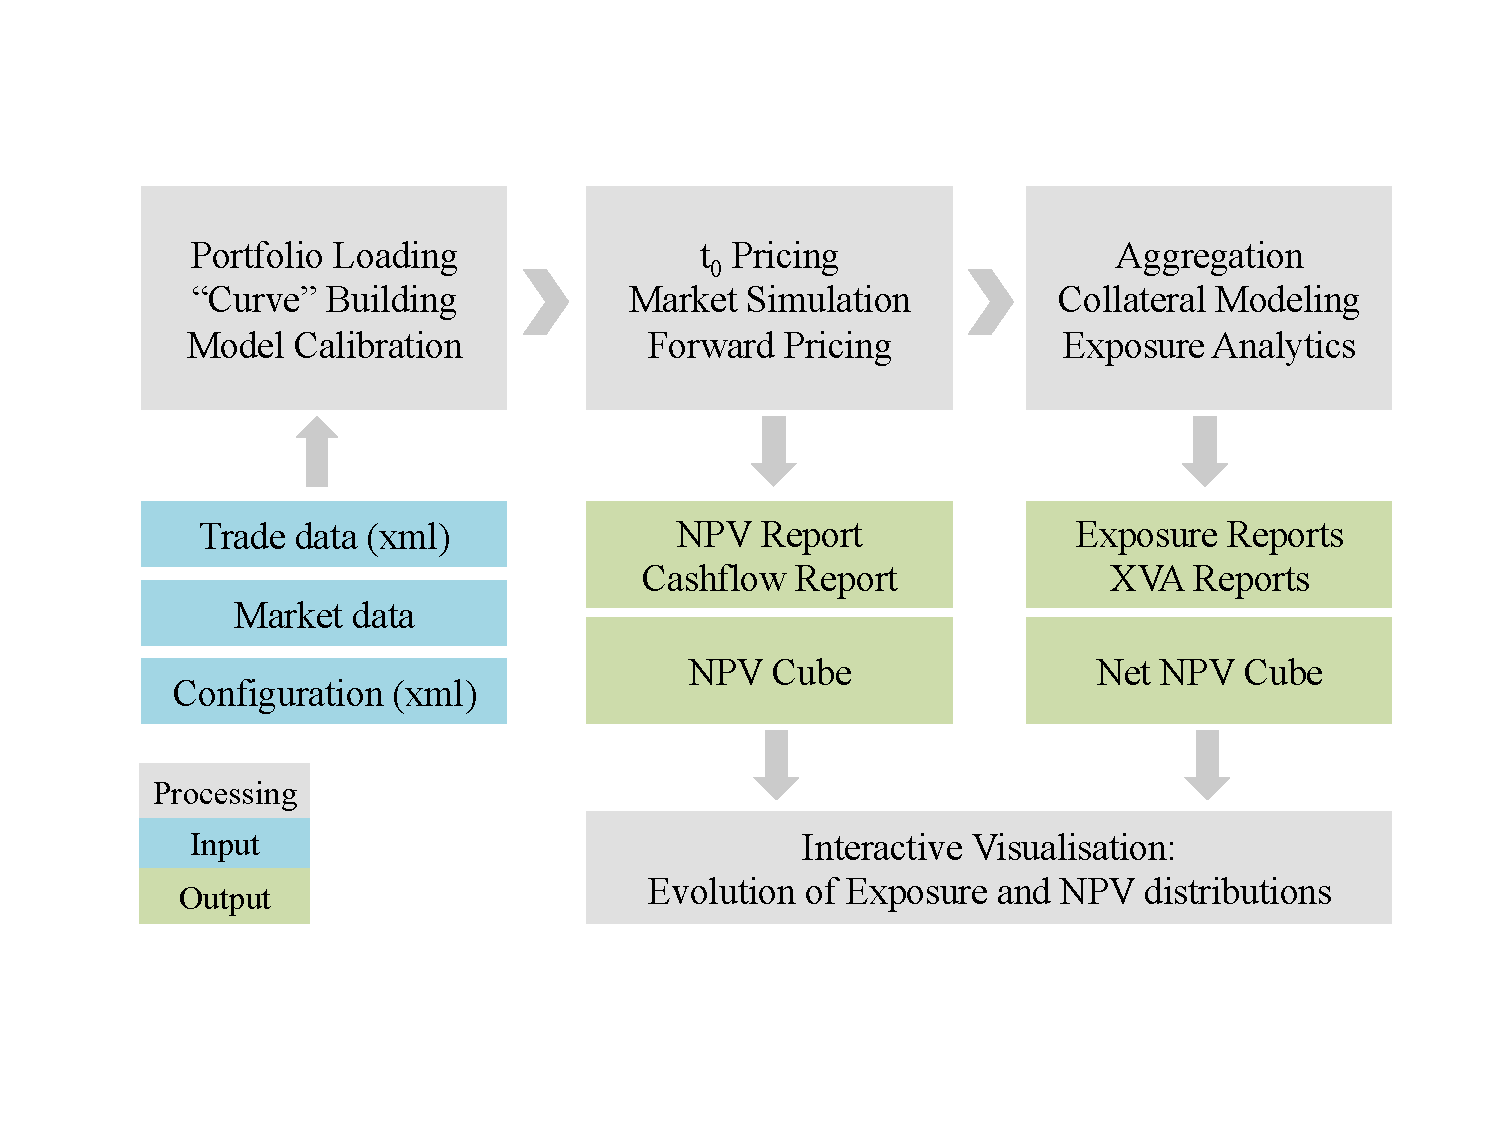
\includegraphics[scale=0.6]{../UserGuide/process.pdf}
\end{center}
\caption{ Information flow implemented in ORE App. }
\label{fig_process}
\end{figure}


\subsection*{Applications}
ORE comes with a command line application that wraps the OREApp class in OREAnalytics, with the following minimal main function.

\begin{listing}[H]
%\hrule\medskip
\begin{minted}[fontsize=\footnotesize]{cpp}
int main(int argc, char** argv) {
	// ...
	if (argc != 2) {
		std::cout << endl << "usage: ORE path/to/ore.xml" << endl << endl;
		return -1;
	}
	string inputFile(argv[1]);
	boost::shared_ptr<Parameters> params = boost::make_shared<Parameters>();
	try {
		params->fromFile(inputFile);
		OREApp ore(params);
		return ore.run();
	} catch (const exception& e) {
		cout << endl << "an error occured: " << e.what() << endl;
		return -1;
	}
}
\end{minted}
\end{listing}

The ORE User Guide at \url{https://opensourcerisk.org/documentation} discusses the usage of the ORE command line application in detail, the main ore.xml input file passed to the application and the various inputs referenced therein.

\subsection*{Unit Tests}
All three libraries - QuantExt, OREData and OREAnalytics - are covered by unit test suites, again following the example of QuantLib. In total the test suites currently
comprise about 430 test cases while the ORE C++ code base size is about 185 thousands source lines of code. This should be compared to QuantLib with about 775 test cases and a code base size of 420 thousand lines, which indicates a code coverage
in ORE that exceeds the coverage in QuantLib.

\subsection*{Language Bindings}
To open ORE up and make its components accessible from other programming languages such as Python and Java, we pursue the same approach as QuantLib and provide (a framework of) language bindings using SWIG, the Simple Wrapper
Interface Generator (\url{http://swig.org}).

\begin{figure}[h]
\begin{center}
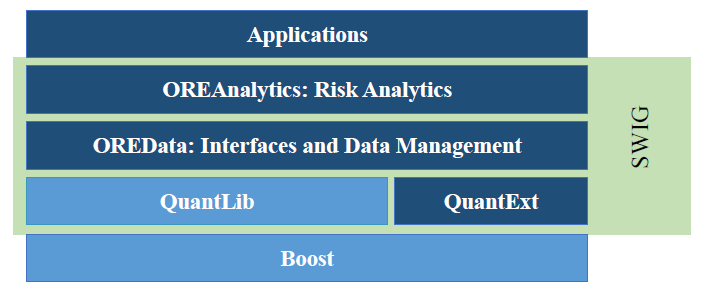
\includegraphics[scale=0.6]{OverviewSWIG}
\end{center}
\caption{SWIG wrapper. }
\label{fig_SWIG}
\end{figure}

The ORE SWIG bindings are open source as well and provided in a separate repository \url{https://github.com/opensourcerisk/ore-swig}). This project provides language bindings for QuantLib, QuantExt, OREData and OREAnalytics as illustrated in figure 
\ref{fig_SWIG}. This allows, for example, running the ORE process that is encapsulated in the C++ call {\tt ore.run()} in Python, but also also allows querying members of the OREApp object in Python or calling into lower level OREData, QuantLib or
QuantExt objects in Python. Refer to the examples in the ORE-SWIG project.

\newpage
\section{QuantExt}
QuantExt collects ORE's extensions to QuantLib such as financial instruments, pricing models, pricing engines and term structures, to achieve the product coverage across six
asset classes ORE is aiming for. The internal organization of QuantExt (folder structure, class hierarchy) mimics the structure of QuantLib, so that a developer who is familiar with QuantLib will have little difficulty finding her/his way around QuantExt as well.
Moreover we follow closely the design of QuantLib since
\begin{itemize}
\item QuantLib's design is based on decades of quant developer experience and well tested in practice over the past 20 years
\item we want to keep the option open that QuantExt code is migrated in part or entirely into QuantLib in the future
\end{itemize}

We do not elaborate on the QuantLib/QuantExt design and patterns, or the range of basic QuantLib objects here as this has been well covered by Luigi Ballabio, one of QuantLib's creators, in his reference book ``Implementing QuantLib - Quantitative finance in C++: an inside look at the architecture of the QuantLib library''
(\url{https://leanpub.com/implementingquantlib}) with free drafts available in his blog posts on \url{https://www.implementingquantlib.com}.
In the following we sketch the current scope of the QuantLib extensions in QuantExt, as of the time of writing this text (November 2019). 
This concrete list is continuously growing and will be out of date at the time of the next release, i.e. check the on-line documentation at \url{https://www.opensourcerisk.org/docs/qle/index.html} for an up-to-date picture.

\begin{itemize}
\item {\bf Calendars}: Chile, Colombia, France, Israel, Malaysia, Netherlands, Peru, Philippines, Switzerland, Thailand
\item {\bf Cashflows}: Average overnight indexed coupon and pricer, BRL CDI coupon pricer, Equity coupon and pricer, floating annuity coupon and pricer, FX linked notional coupon and cashflow, log-normal CMS spread pricer, Quanto coupon pricer, stripped capped/floored YOY inflation coupon, sub-period coupon and pricer
\item {\bf Currencies}: Africa (TND, EGP, NGN, MAD), America (MXV, CLF), Asia (KZT, QAR, BHD, OMR, AED, PHP, CNH), Precious Metals (XAU, XAG, XPT, XPD)
\item {\bf Indexes}: Bond index, Commodity index, Equity index, FX index, Inflation indices (CA CPI, Danish CPI, Swedish CPI), and a range of 40 IBOR indices connected with the additional currencies above
\item {\bf Instruments}: 24 instrument classes - Average OIS, BRL CDI Swap, CDS Option, Commodity Forward, Credit Default Swap, Cross Currency Basis MTM Reset Swap, Cross Currency Basis Swap, Cross Currency Fixed/Float Swap, Cross Currency Swap, Currency Swap, Deposit, Equity Forward, Fixed BMA Swap, Forward Bond, FX Forward, Implied Bond Spread Helper, OIS Basis Swap, Overnight Indexed Cross Currency Basis Swap, Sub Periods Swap, Tenor Basis Swap
\item {\bf Math}: Delta Gamma VaR, Nadaraya Watson Regression, Stabilized General Linear Least Squares Fit
\item {\bf Monte Carlo Methods}: Multi Path Generator
\item {\bf Models}: 32 model and model parameterization helper classes - Linear Gauss Markov Model (LGM), Cross Asset Model, Cross Asset Analytics, Cross Asset Model Parametrization (EQ BS Constant / Piecewise Constant, FX BS Constant/ Piecewise Constant, IR LGM1F Constant / Piecewise Linear / Constant HullWhite, INF DK, CR LGM1F),Calibration Helpers (CMS Cap, CPI Cap/Floor, CDS Option, FX/EQ Option), Model Implied Termstructures (DK Zero Inflation, DK YOY Inflation, LGM Credit, LGM Yield), Linkable Calibrated Model
\item {\bf Pricing Engines}: 24 pricing engines covering the additional instruments above - Analytic Cross Currency LGM FX Option, Analytic DK CPI Cap/Floor, Analytic LGM CDS Option, Analytic LGM Swaption, Analytic Cross Asset LGM Equity Option, Barone Adesi Whaley, Black CDS Option, CPI Bachelier Cap/Floor, CPI Black Cap/Floor, Cross Currency Swap, Deposit, Commodity Forward, Currency Swap, Equity Forward, FX Forward, Risky Bond, Swap Delta, Swap Multi Curve, LGM Convolution Solver, Midpoint CDS, Numeric LGM Swaption, Overnight Index Cross Currency Basis Swap
\item {\bf Processes}: Cross Asset State Process, IR LGM1F State Process
\item {\bf Quotes}: Log Quote
\item {\bf Term Structures}: 80 term structures and helper classes supporting the pricing across six asset classes -
\begin{itemize}
\item {\bf Bootstrap Helpers}: Average OIS Rate Helper, Basis Two Swap Helper, BRL CDI Rate Helper, Cap/Floor Helper, Cross Currency Basis MTM Reset Swap Helper, Cross Currency Basis Swap Helper, Cross Currency Fix/Float Swap Helper, IMM FRA Rate Helper, Dated Stripped Optionlet and Adapter, Default Probability Helpers, Equity Forward Curve Stripper, Overnight Index Basis Swap / Cross Currency Basis Swap, Sub-Periods Swap, Tenor Basis Swap
\item {\bf Black Volatility Term Structures}: Inverted Vol, Monotone Variance, Variance Moneyness, Surface with Delta, Surface with ATM, Sparse Surface, 
\item {\bf Dynamic Termstructures}: Black Vol Termstructure, Optionlet Vol Termstructure, Swaption Vol Matrix, YOY Optionlet Vol Termstructure
\item {\bf Spreaded Termstructures}: Spreaded Optionlet Volatility, Spreaded Smile Section, Spreaded Swaption Volatility, Equity Vol Constant Spread, Hazard Spreaded Default Termstructure
\item {\bf FX}: Black Vol Surface, Smile Section, Vanna Volga Smile Section
\item {\bf Inflation}: Stripped CPI Volatility Structure, Stripped YOY Inflation Optionlet Volatility, YOY Inflation Optionlet Stripper, YOY Optionlet Volatility Surface, corrections of QuantLib's ``KInterpolatedYoYOptionletVolatilitySurface''
\item {\bf Correlation}: Correlation Termstructure, Flat Correlation Termstructure
\item {\bf Others}: Cap/Floor Term Vol Curve, Cap/Floor Term Vol Surface, Cross Currency Price Termstructure, Discount Ratio Modified Curves, Price Term Structure and Adapter, Extension of QuantLib's Iterative Bootstrap, corrections and extensions to QuantLib's Optionlet Stripper
\end{itemize}
\item {\bf Time}: Year Counter, Futures Expiry Calculator
\end{itemize}

The current size of the QuantExt code base is about 77 thousand source lines (excluding blank lines), of 185 thousand lines in total across the three libraries in ORE.

\newpage
\section{Data}
The Data management library OREData, as stated above, hosts the classes for
\begin{itemize}
\item translating external trade, market and configuration data into financial objects that QuantExt and QuantLib can deal with, and
\item assembling these into object hierarchies the higher level analytics can use  conveniently (e.g. Portfolio, Market, Pricing Models, Simulation Models)
\end{itemize}

The OREData library currently comprises about 78 thousand lines of code, close to the size of QuantExt.

We start illustrating OREData's design by focusing on the Market objects.

\subsection{Market Data}\label{sec:marketdata}
The market base class provides the interface to all kinds of term structure objects that might be needed in pricing across asset classes. Listing \ref{1st:marketdata} shows a small excerpt, all member functions are pure virtual and are implemented in derived classes. It is then
sufficient to pass a smart pointer respectively Handle to a base Market object into classes or functions that need to perform pricing. Relevant term structures, indices and quotes are queried by providing a single unique key or set of keys.

The Market interface covers
\begin{itemize}
\item Yield term structures by type and name, as shown in listing \ref{1st:marketdata}
\item Swaption volatility structures by currency
\item Discount curves by currency
\item IBOR and Swap indices (with associated forward curves) by index name
\item FX Spot quotes by currency pair
\item FX volatility term structures by currency pair
\item Default term structures by name
\item Recovery rate quotes by name
\item CDS volatility term structures by name
\item Base correlation term structures by qualifier
\item Zero and Year-on-Year inflation indices (with associated forward curves) by index name
\item Cap/Floor volatility structures by currency
\item Year on year Cap/Floor volatility and price surfaces by index name
\item Zero inflation Cap/Floor volatility and price surfaces by index name
\item Equity spot prices, dividend and forecasting curves by equity name
\item Equity volatility term structures by equity name
\item Security spreads by security ID
\item Commodity price curves by commodity name
\item Commodity volatility term structures by commodity name
\item Generic correlation term structures by index pair
\item Prepayment rate quotes by security ID
\end{itemize}

\begin{listing}[H]
%\hrule\medskip
\begin{minted}[fontsize=\footnotesize]{cpp}
class Market {
public:
virtual ~Market() {}
virtual Date asofDate() const = 0;
//! \name Yield Curves
//@{
virtual Handle<YieldTermStructure>
discountCurve(const string& ccy,
const string& configuration = Market::defaultConfiguration) const = 0;
virtual Handle<IborIndex>
iborIndex(const string& indexName,
const string& configuration = Market::defaultConfiguration) const = 0;
virtual Handle<SwapIndex>
swapIndex(const string& indexName,
const string& configuration = Market::defaultConfiguration) const = 0;
//@}
//! \name Swaptions
//@{
virtual Handle<SwaptionVolatilityStructure>
swaptionVol(const string& ccy,
const string& configuration = Market::defaultConfiguration) const = 0;
// ...
//@}
//! \name Foreign Exchange
// ...
};
\end{minted}
\caption{Market base class, pure virtual member functions with varying number and type of keys and common last argument indicating the ``curve ID'' to select one of several market configurations.}
\label{1st:marketdata}
\end{listing}

The {\tt MarketImpl} class is derived from {\tt Market}, and it essentially provides member variables (maps) to store the underlying term structures, indices and quotes.
The {\tt TodaysMarket} class is derived from {\tt MarketImpl}, and it provides a constructor that builds a concrete Market instance. 
This build process involves various helper classes for each term structure across the asset classes, see folder {\tt OREData/ored/marketdata}, as well as configuration helpers for each term structure in folder {\tt OREData/ored/configuration}. Moreover, the build process involves
\begin{itemize}
\item reading market data in csv files and term structure configurations data XML files into internal data classes, and
\item parsing/translating text into basic QuantLib/QuantExt objects such as Calendars, Periods, Currencies, Quotes etc., all supported by the utility code assembled in folder {\tt OREData/ored/utilities}.
\end{itemize}
The {\tt TodaysMarket} class is sufficient for portfolio pricing. Further derived classes that are essential for market simulation and scenario analysis are introduced in the next section on OREAnalytics.

\subsection{Portfolio and CSA Data}

\begin{listing}[H]
%\hrule\medskip
\begin{minted}[fontsize=\footnotesize]{cpp}
class Portfolio {
public:
//! Get a Trade with the given trade id from the portfolio
boost::shared_ptr<Trade> get(const std::string& id) const;
//! Load using a default or user supplied TradeFactory
void load(const std::string& fileName,
const boost::shared_ptr<TradeFactory>& tf = boost::make_shared<TradeFactory>());
//! Load from an XML string using a default or user supplied TradeFactory
void loadFromXMLString(const std::string& xmlString,
const boost::shared_ptr<TradeFactory>& tf
= boost::make_shared<TradeFactory>());
//! Load from XML Node
void fromXML(XMLNode* node,
const boost::shared_ptr<TradeFactory>& tf
= boost::make_shared<TradeFactory>());
//! Save portfolio to an XML file
void save(const std::string& fileName) const;
//! Call build on all trades in the portfolio
void build(const boost::shared_ptr<EngineFactory>&);
//! Return trade list
const std::vector<boost::shared_ptr<Trade>>& trades() const { return trades_; }
// ...
};
\end{minted}
\caption{Excerpt of the Portfolio class showing essential member functions.}
\label{1st:portfolio}
\end{listing}

The second large part of OREData deals with trade loading and building from external sources and assembling all trades in a {\tt Portfolio} object. An excerpt is shown in listing \ref{1st:portfolio}. The {\tt Portfolio} class provides several ways of loading a portfolio (from an
XML file, an XML string, a single XML node), to store a portfolio to XML file, to access individual trades. When a portfolio is loaded from an external source, it is first represented in internal trade objects where all relevant fields are native (string, integer, double, bool) variables
or standard C++ containers like vectors or maps.

In a subsequent step, initiated by a call to the {\tt build} member function, the ``raw'' trade data is then translated into QuantLib/QuantExt objects up to the QuantLib/QuantExt instrument, linked to a QuantLib/QuantExt pricing engine, in turn linked to the relevant term structures provided by the {\tt Market} class introduced in Section \ref{sec:marketdata}.
The role of the {\tt TradeFactory} class in the Portfolio member functions is to help constructing concrete instances of trade objects depending on the TradeType information in the trade XML representation.
All trade objects derive from a common {\tt Trade} base class shown in listing \ref{1st:trade}.

\begin{listing}[H]
%\hrule\medskip
\begin{minted}[fontsize=\footnotesize]{cpp}
class Trade {
public:
class Trade : public XMLSerializable {
public:
// Constructor
// ....
//! Build QuantLib/QuantExt instrument, link pricing engine
virtual void build(const boost::shared_ptr<EngineFactory>&) = 0;
//! Return fixings that are relevant for pricing
virtual std::map<std::string, std::set<QuantLib::Date>>
fixings(const QuantLib::Date& settlementDate = QuantLib::Date()) const = 0;
//! \name Serialisation
//@{
virtual void fromXML(XMLNode* node);
virtual XMLNode* toXML(XMLDocument& doc);
//@}
//! \name Inspectors
//@{
const string& id() const { return id_; }
const string& tradeType() const { return tradeType_; }
const Envelope& envelope() const { return envelope_; }
const set<string>& portfolioIds() const { return envelope().portfolioIds(); }
const TradeActions& tradeActions() const { return tradeActions_; }
const boost::shared_ptr<InstrumentWrapper>& instrument() { return instrument_; }
const std::vector<QuantLib::Leg>& legs() { return legs_; }
const std::vector<string>& legCurrencies() { return legCurrencies_; }
const std::vector<bool>& legPayers() { return legPayers_; }
const string& npvCurrency() { return npvCurrency_; }
const Date& maturity() { return maturity_; }
//@}
//...
};
\end{minted}
\caption{Excerpt of the Trade class showing essential member functions.}
\label{1st:trade}
\end{listing}

The {\tt Trade} class provides access to the underlying QuantLib/QuantExt instrument and further trade information that is meaningful across all kinds of products. There is a range of concrete classes derived from {\tt Trade} that perform the actual load and build process, see folder {\tt OREData/ored/portfolio}, currently
\begin{itemize}
\item Bond
\item Cap/Floor
\item Commodity Forward, European Commodity Option
\item Credit Default Swap
\item Equity Forward, Equity Swap, European Equity Option
\item Forward Bond
\item Forward Rate Agreement
\item FX Forward, FX Swap, European and American FX Option
\item Swap
\item European and Bermudan Swaption
\end{itemize}

The trade design is modular, and objects re-used within various trade types as member variables are
\begin{itemize}
\item Envelope
\item Schedule
\item OptionData
\item LegData
\item TradeActions
\end{itemize}
each of which comes with functions for loading from XML, building QuantLib/QuantExt objects.

{\bf CSA Data} is represented in a single class, {\tt NettingSetDefinition}, see folder {\tt OREData/ored/portfolio}, also XML serializable like each trade. The ``portfolio'' of CSAs is then managed by class {\tt NettingSetManager}, 
XML serializable like the {\tt Portfolio} object.

\subsection{Pricing Engines, Engine Factory}
Each trade is linked with a pricing engine during the trade's build process. In order to limit the number of engines to be constructed (and to limit memory usage), ORE reuses engines as far as possible. This is achieved by the {\tt EngineBuilder},
{\tt EngineFactory} and {\tt LegBuilder} classes. Currently, ORE provides 36 concrete ``default'' engine and leg builders when the {\tt EngineFacotry} is constructed. The design here is extensible so that a developer can add his/her own engine builders to the
factory when extending ORE. For this purpose the {\tt EngineFactory} class provides the {\tt addExtraBuilders} member function.

Figure \ref{fig_OREDPortfolio} shows the relationships of these classes:

\begin{figure}[h]
\begin{center}
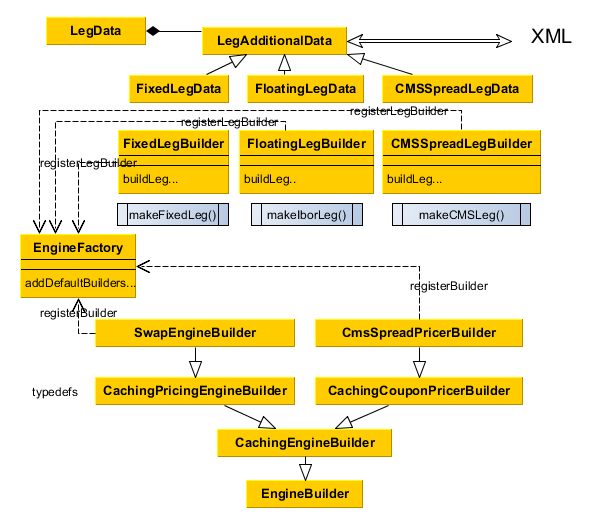
\includegraphics[scale=0.6]{ORED_Portfolio}
\end{center}
\caption{Collaboration Diagram of Instrument/Leg Builder and Factory Classes}
\label{fig_OREDPortfolio}
\end{figure}

\subsection{Pricing Models and Simulation Models}
The construction and calibration of Pricing and Simulation models is encapsulated in the {\tt LgmBuilder} and {\tt CrossAssetModelBuilder} classes, see folder {\tt OREData/ored/models}. Both are supported by associated ``data'' classes that hold
the model/calibration configuration, XML serializable like portfolio and other configuration data in ORE.

\newpage
\section{Analytics}
The OREAnalytics library comprises the classes for portfolio risk analytics, in particular Monte Carlo simulation-based analytics. It was originally designed to support exposure simulation and XVA, but also covers hypothetical scenario analysis
(sensitivities, stress testing). The classes in OREAnalytics depend on QuantLib, QuantExt and OREData, and the primary inputs into analytics are the Portfolio, Market and CrossAssetModel objects introduced in section \ref{sec:marketdata}
The OREAnalytics library currently comprises about 30 thousand lines of code.

\subsection{Simulation Market}
The {\tt TodaysMarket} class in OREData provides a snapshot of the market as of a given reference date. The Portfolio is linked to this market to produce the reference date's valuations and cash flow projections. ORE's design to support analysis of how
valuations change when the market moves under hypothetical scenarios with fixed reference date or under market changes through time is to ``simply'' link the portfolio to a market that change in these ways and then triggers repricing. 
The key element for the implementation is the {\tt SimMarket} class, derived from the {\tt MarketImpl} (which is derived form {\tt Market}), i.e. it provides the same interfaces, and some additional and essential member functions, 
in particular the {\tt update} function, as shown in listing \ref{1st:simmarket}, see folder {\tt OREAnalytics/orea/simulation}.

\begin{listing}[H]
%\hrule\medskip
\begin{minted}[fontsize=\footnotesize]{cpp}
class SimMarket : public data::MarketImpl {
public:
SimMarket(const Conventions& conventions) : MarketImpl(conventions), numeraire_(1.0) {}
//! Generate or retrieve market scenario, update market, notify termstructures and update fixings
virtual void update(const Date&) = 0;
//! Return current numeraire value
Real numeraire() { return numeraire_; }
//! Reset sim market to initial state
virtual void reset() = 0;
//! Get the fixing manager
virtual const boost::shared_ptr<FixingManager>& fixingManager() const = 0;
protected:
Real numeraire_;
};
\end{minted}
\caption{Simulation Market base class.}
\label{1st:simmarket}
\end{listing}

The concrete class that derives from {\tt SimMarket} and that actually implements {\tt update}, {\tt reset} and {\tt fixingManager} is {\tt ScenarioSimMarket}, as shown in listing \ref{1st:scenariosimmarket}, see folder {\tt OREAnalytics/orea/scenario}.

\begin{listing}[H]
%\hrule\medskip
\begin{minted}[fontsize=\footnotesize]{cpp}
//! Simulation Market updated with discrete scenarios
class ScenarioSimMarket : public analytics::SimMarket {
public:
//! Constructors
// ...
//! Set scenario generator
boost::shared_ptr<ScenarioGenerator>& scenarioGenerator() { return scenarioGenerator_; }
//! Set aggregation data
boost::shared_ptr<AggregationScenarioData>& aggregationScenarioData() { return asd_; }
//! Set scenarioFilter
boost::shared_ptr<ScenarioFilter>& filter() { return filter_; }
//! Update market snapshot and relevant fixing history
void update(const Date& d) override;
//! Reset sim market to initial state
virtual void reset() override;
//! Return the fixing manager
const boost::shared_ptr<FixingManager>& fixingManager() const override { return fixingManager_; }
// ...
};
\end{minted}
\caption{Excerpt of the concrete Simulation Market class.}
\label{1st:scenariosimmarket}
\end{listing}

The {\tt ScenarioGenerator} class that appears here is used to generate single or multiple market Scenarios. This is used in ScenarioSimMarket's {\tt update} function which then
applies the generated scenario to the underlying data in {\tt ScenarioSimMarket}. Moreover, the update call triggers QuantLib observer notification chains so that the portfolio that is linked to {\tt ScenarioSimMarket} reacts to these changes with amended
valuations when asked for NPVs next time. To finish this section we note that the configuration for the simulation market's composition is externally done in ORE XML, and there is a configuration class {\tt ScenarioSimMarketParameters} which is XML (de-)serializable, and used in the construction of the {\tt ScenarioSimMarket} object.

\subsection{Scenario Generation}
OREAnalytics covers two types of Monte Carlo scenario generators that produce market evolutions - {\tt LgmScenarioGenerator} for risk neutral interest rate scenarios only,
{\tt CrossAssetModelScenarioGenerator} for IR/FX/INF/EQ market scenarios, as well as sensitivity and stress testing scenario generators {\tt SensitivityScenarioGenerator} and {\tt stressScenarioGenerator}. 
All generators have associated XML (de-)serializable configuration classes which are used to construct the generators. 
The interface between any scenario generator and the {\tt ScenarioSimMarket} is the {\tt Scenario} object shown in listing \ref{1st:scenario}. Its concrete derived classes hold the actual generated data.

\begin{listing}[H]
%\hrule\medskip
\begin{minted}[fontsize=\footnotesize]{cpp}
class Scenario {
public:
//! Return the scenario asof date
virtual const Date& asof() const = 0;
//! Get the scenario label
virtual const string& label() const = 0;
//! Set the scenario label
virtual void label(const string&) = 0;
//! Get Numeraire ratio n = N(t) / N(0) so that Price(0) = N(0) * E [Price(t) / N(t) ]
virtual Real getNumeraire() const = 0;
//! Set the Numeraire ratio n = N(t) / N(0) so that Price(0) = N(0) * E [Price(t) / N(t) ]
virtual void setNumeraire(Real n) = 0;
//! Check whether this scenario provides the data for the given key
virtual bool has(const RiskFactorKey& key) const = 0;
//! Risk factor keys for which this scenario provides data
virtual const std::vector<RiskFactorKey>& keys() const = 0;
//! Add an element to the scenario
virtual void add(const RiskFactorKey& key, Real value) = 0;
//! Get an element from the scenario
virtual Real get(const RiskFactorKey& key) const = 0;
//! clones a scenario and returns a pointer to the new object
virtual boost::shared_ptr<Scenario> clone() const = 0;
// ...
};
\end{minted}
\caption{Excerpt of the Scenario data class.}
\label{1st:scenario}
\end{listing}

The scenario object refers to a unique reference date and contains an arbitrarily large number of data points that are identified by a RiskFactorKey. The key identifies the risk factor class (25 types so far in ORE, see the definition in
{\tt OREAnalytics/orea/scenario/scenario.hpp}, e.g. {\tt DiscoutCurve}, {\tt IndexCurve}, {\tt SwaptionVolatility}, etc.), a name (e.g. a currency or index name), and an integer indicating the position of the data item in a vector, matrix or cube. A market
evolution or path is hence represented by a vector of scenarios. So far there is only one derived class from the base Scenario in ORE, {\tt SimpleScenario}, which stores the scenario data in simple vectors and maps, also serializable.

\subsection{Engine}
The {\tt OREAnalytics/orea/engine} folder comprises a number of calculators (wrapped into individual classes) for ORE's risk analytics beyond single pricing as of the reference date:
\begin{itemize}
\item ValuationEngine - performs a market simulation, prices a portfolio under scenarios, possibly through time, and fills a resulting NPV cube, with the help of the ValuationCalculator class; the ValuationEngine is used for Monte Carlo simulations of the market evolution but also the hypothetical scenario analytics below
\item SensitivityAnalysis, also performed with the help of ValuationEngine and ValuationCalculator: This class wraps functionality to perform a sensitivity analysis for a given portfolio.
\begin{itemize}
\item builds the "simulation" market to which sensitivity scenarios are applied, 
\item builds the portfolio linked to this simulation market
\item generates sensitivity scenarios
\item runs the scenario "engine" to apply these and compute the NPV impacts of all required shifts
\item compiles first and second order sensitivities for all factors and all trades
\item fills result structures that can be queried
\end{itemize}
\item StressTest, also performed with the help of ValuationEngine and ValuationCalculator: This class wraps functionality to perform a stress testing analysis for a given portfolio and
\begin{itemize}
\item builds the "simulation" market to which stress scenarios are applied, 
\item builds the portfolio linked to this simulation market
\item generates stress scenarios
\item runs the scenario "engine" to apply these and compute the NPV impacts of all required shifts
\item fills result structures that can be queried
\item writes stress test report to a file
\end{itemize}
\item ParametricVarCalculator, as post-processor of a SensitivityStream, takes sensitivity data and a covariance matrix as an input and computes a parametric value at risk. The output can be broken down by portfolios, risk classes (IR, FX, EQ, ...) and risk types (delta-gamma, vega, ...)
\item CounterpartyCalculator/SurvivalProbabilityCalculator, calculates the survival probability of a counterpart to be stored in the resulting cube
\end{itemize}

\subsection{Aggregation, Cubes, XVA and Post Process}
For the calculation of XVA and exposures, ORE first applies the {\tt ValuationEngine} above to build the required cubes (NPV cube on Nettingset level and trade level, Cpty Cube for survival probabilities), this is done in method {\tt buildCube}.

The resulting cubes contain NPVs per Trade/Nettingset, future evaluation date and scenario. The cubes are then passed into the {\tt PostProcess} class (see folder {\tt OREAnalytics/ore/aggregation}).

The post processor is an orchestrating class performing following tasks (XML configurable) for the full portfolio and associated cube:
\begin{itemize}
\item compute netting set NPVs as of the reference date and find each netting set's maturity
\item aggregate NPVs across trades per netting set, construct an NPV cube by netting set, future valuation date and scenario
\item apply ORE's regression based dynamic initial margin model to project future Initial Margin per netting set and Monte Carlo path
\item generate exposure evolutions per trade (expected positive and negative exposures, potential future exposures, etc.) without collateral
\item generate collateral account balance evolutions per netting set, using CSA details in each NettingSet object (thresholds, minimum transfer amounts, independent amounts etc.)
\item generate netting set exposure evolutions (after collateral)
\item allocate netting set exposures to trade level
\item compute XVAs (CVA, DVA, FCA, FBA, MVA, KVA) each netting set
\item allocate netting set XVAs to trade level, excluding KVA
\end{itemize}

The {\tt PostProcess} class does these tasks with the help of other classes (see folder {\tt OREAnalytics/ore/aggregation}):

\begin{itemize}
\item {\tt ValueAdjustmentCalculator}/ {\tt StaticCreditXvaCalculator}/ {\tt DynamicCreditXvaCalculator}: ValueAdjustmentCalculator defines an interface for derived classes to to perform the XVA calculations for all netting sets and along all paths. StaticCreditXvaCalculator calculates xva using survival probability from market, DynamicCreditXvaCalculator calculates xva using survival probability from each path
\item {\tt RegressionDynamicInitialMarginCalculator}/ {\tt DynamicInitialMarginCalculator}: Dynamic Initial Margin calculation, fills DIM cube per netting set that can be
\begin{itemize}
\item returned to be further analyzed
\item used in collateral calculation
\item used in MVA calculation
\end{itemize}
\item {\tt ExposureCalculator}: Trade Exposure and Netting
\begin{itemize}
\item Aggregation across scenarios per trade and date. This yields single trade exposure profiles, EPE and ENE
\item Aggregation of NPVs within netting sets per date and scenario. This prepares the netting set exposure calculation below
\end{itemize}
\item {\tt NettedExposureCalculator}: Netting set exposure and allocation to trades
\begin{itemize}
\item Compute all netting set exposure profiles EPE and ENE using collateral if CSAs are given and active.
\item Compute the expected collateral balance for each netting set.
\item Allocate each netting set's exposure profile to the trade level such that the trade exposures add up to the netting set exposure.
\end{itemize}
\item {\tt ExposureAllocator}/ {\tt RelativeFairValueNetExposureAllocator}/ {\tt RelativeFairValueGrossExposureAllocator}/ {\tt RelativeXvaExposureAllocator}/ {\tt NoneExposureAllocator}: calculates EPE/ENE based on selected AllocationMethod
\item {\tt CollateralExposureHelper}: This class contains helper functions to aid in the calculation of collateralised exposures. It can be used to calculate margin requirements in the presence of e.g. thresholds and minimum transfer amounts, update collateral account details with e.g. new margin call info, and return collateralised exposures to the user/invoker.
\item {\tt CollateralAccount}: This class holds information corresponding to collateral cash accounts. It stores a balance as well as an asof date for the balance. The class also includes "margin" information relating to the most recent margin call (e.g. call amount, status, expected pay date. The idea is that this class can be updated on-the-run with new margin requirements and collateral balances, and the timestamps updated accordingly.
\item {\tt CVASpreadSensitivityCalculator}: Compute hazard rate and CDS spread sensitivities for a given exposure profile on an externally provided sensitivity grid.
\end{itemize}

\subsection{Orchestration, ORE App}
Finally, all analytics described above are orchestrated by a single class {\tt OREApp}, see folder {\tt OREAnalytics/orea/app}. This includes
\begin{itemize}
\item loading and building the initial market
\item building the engine factory
\item loading and building of the portfolio
\item generating cash flow, NPV and curve reports
\item performing sensitivity analysis
\item performing stress tests
\item performing parametric VaR calculations
\item running the Monte Carlo simulation to build an NPV cube
\item performing cube aggregation, post-processing steps
\item generating exposure and XVA reports
\item generating a dynamic Initial Margin report
\end{itemize}

Which analytics are run and their parameterization is XML configurable, see class {\tt Parameters}. Report generation is supported by the {\tt ReportWriter} class in folder {\tt OREAnalytics/orea/app} and the {\tt Report} class in folder {\tt OREData/ored/report}.

The Sensitivity Analysis is performed by the class {\tt SensitivityRunner}.

XVA Analysis can be done in two ways:

In case the XVA simulation should be run in one go, the class {\tt XvaRunner} can be used:

\begin{listing}[H]
%\hrule\medskip
\begin{minted}[fontsize=\footnotesize]{cpp}
	boost::shared_ptr<XvaRunner> xva = getXvaRunner();
	xva->runXva(market_, true);
	postProcess_ = xva->postProcess();
	writeXVAReports();
	if (writeDIMReport_)
		writeDIMReport();
\end{minted}
\caption{Usage of the XvaRunner class.}
\label{1st:XvaRunner}
\end{listing}

Otherwise, the simulation can be separated from the XVA calculation:

\begin{listing}[H]
%\hrule\medskip
\begin{minted}[fontsize=\footnotesize]{cpp}
	if (simulate_) {
		generateNPVCube();
	} else {
		LOG("skip simulation");
	}

	if (xva_) {
		// We reset this here because the date grid building below depends on it.
		Settings::instance().evaluationDate() = asof_;
		// Use pre-generated cube
		if (!cube_)
			loadCube();
		// Use pre-generated scenarios
		if (!scenarioData_)
			loadScenarioData();
		runPostProcessor();
		writeXVAReports();
		if (writeDIMReport_)
			writeDIMReport();
	} else {
		LOG("skip XVA reports");
	}
\end{minted}
\caption{separate simulation and calculation of XVA.}
\label{1st:SeparateSimXVA}
\end{listing}

\section{Unit Tests}
All three ORE libraries (QuantExt, OREData and OREAnalytics) are covered by respective unit test suites with source code in folders
\begin{itemize}
\item {\tt QuantExt/test}
\item {\tt OREData/test}
\item {\tt OREAnalytics/test}
\end{itemize}
with currently 132 test cases in QuantExt, 254 test cases in OREData and 43 test cases in OREAnalytics. Test suites are continuously extended when new functionality is added or when a bug is identified and fixed.

\section{Language Bindings}
The ORE language bindings are built following the QuantLib example using SWIG. The framework provided in the separate repository
\url{https://github.com/opensourcerisk/ore-swig}) covers a subset of the ORE classes and member functions so far. The initial goal of the ORE-SWIG project was to provide a working framework with focus on Python support that allows access to
classes and functions across all ORE libraries including QuantLib within a single Python module. This has been achieved with the May 2019 release. We expect that coverage will be extended over the course of the next releases. Because of the
community's expressed interest in Python bindings, we expect contributions from the ORE community over time.

\end{document}
